\documentclass[11pt,preprint, authoryear]{elsarticle}

\makeatletter
\renewcommand\@biblabel[1]{}
\makeatother

\usepackage{lmodern}
%%%% My spacing
\usepackage{setspace}
\setstretch{1.2}
\DeclareMathSizes{12}{14}{10}{10}

% Wrap around which gives all figures included the [H] command, or places it "here". This can be tedious to code in Rmarkdown.
\usepackage{float}
\let\origfigure\figure
\let\endorigfigure\endfigure
\renewenvironment{figure}[1][2] {
    \expandafter\origfigure\expandafter[H]
} {
    \endorigfigure
}

\let\origtable\table
\let\endorigtable\endtable
\renewenvironment{table}[1][2] {
    \expandafter\origtable\expandafter[H]
} {
    \endorigtable
}


\usepackage{ifxetex,ifluatex}
\usepackage{fixltx2e} % provides \textsubscript
\ifnum 0\ifxetex 1\fi\ifluatex 1\fi=0 % if pdftex
  \usepackage[T1]{fontenc}
  \usepackage[utf8]{inputenc}
\else % if luatex or xelatex
  \ifxetex
    \usepackage{mathspec}
    \usepackage{xltxtra,xunicode}
  \else
    \usepackage{fontspec}
  \fi
  \defaultfontfeatures{Mapping=tex-text,Scale=MatchLowercase}
  \newcommand{\euro}{€}
\fi

\usepackage{amssymb, amsmath, amsthm, amsfonts}

\def\bibsection{\section*{References}} %%% Make "References" appear before bibliography


\usepackage[round]{natbib}

\usepackage{longtable}
\usepackage[margin=2.3cm,bottom=2cm,top=2.5cm, includefoot]{geometry}
\usepackage{fancyhdr}
\usepackage[bottom, hang, flushmargin]{footmisc}
\usepackage{graphicx}
\numberwithin{equation}{section}
\numberwithin{figure}{section}
\numberwithin{table}{section}
\setlength{\parindent}{0cm}
\setlength{\parskip}{1.3ex plus 0.5ex minus 0.3ex}
\usepackage{textcomp}
\renewcommand{\headrulewidth}{0.2pt}
\renewcommand{\footrulewidth}{0.3pt}

\usepackage{array}
\newcolumntype{x}[1]{>{\centering\arraybackslash\hspace{0pt}}p{#1}}

%%%%  Remove the "preprint submitted to" part. Don't worry about this either, it just looks better without it:
\makeatletter
\def\ps@pprintTitle{%
  \let\@oddhead\@empty
  \let\@evenhead\@empty
  \let\@oddfoot\@empty
  \let\@evenfoot\@oddfoot
}
\makeatother

 \def\tightlist{} % This allows for subbullets!

\usepackage{hyperref}
\hypersetup{breaklinks=true,
            bookmarks=true,
            colorlinks=true,
            citecolor=blue,
            urlcolor=blue,
            linkcolor=blue,
            pdfborder={0 0 0}}


% The following packages allow huxtable to work:
\usepackage{siunitx}
\usepackage{multirow}
\usepackage{hhline}
\usepackage{calc}
\usepackage{tabularx}
\usepackage{booktabs}
\usepackage{caption}


\newenvironment{columns}[1][]{}{}

\newenvironment{column}[1]{\begin{minipage}{#1}\ignorespaces}{%
\end{minipage}
\ifhmode\unskip\fi
\aftergroup\useignorespacesandallpars}

\def\useignorespacesandallpars#1\ignorespaces\fi{%
#1\fi\ignorespacesandallpars}

\makeatletter
\def\ignorespacesandallpars{%
  \@ifnextchar\par
    {\expandafter\ignorespacesandallpars\@gobble}%
    {}%
}
\makeatother

\newlength{\cslhangindent}
\setlength{\cslhangindent}{1.5em}
\newenvironment{CSLReferences}%
  {\setlength{\parindent}{0pt}%
  \everypar{\setlength{\hangindent}{\cslhangindent}}\ignorespaces}%
  {\par}


\urlstyle{same}  % don't use monospace font for urls
\setlength{\parindent}{0pt}
\setlength{\parskip}{6pt plus 2pt minus 1pt}
\setlength{\emergencystretch}{3em}  % prevent overfull lines
\setcounter{secnumdepth}{5}

%%% Use protect on footnotes to avoid problems with footnotes in titles
\let\rmarkdownfootnote\footnote%
\def\footnote{\protect\rmarkdownfootnote}
\IfFileExists{upquote.sty}{\usepackage{upquote}}{}

%%% Include extra packages specified by user

%%% Hard setting column skips for reports - this ensures greater consistency and control over the length settings in the document.
%% page layout
%% paragraphs
\setlength{\baselineskip}{12pt plus 0pt minus 0pt}
\setlength{\parskip}{12pt plus 0pt minus 0pt}
\setlength{\parindent}{0pt plus 0pt minus 0pt}
%% floats
\setlength{\floatsep}{12pt plus 0 pt minus 0pt}
\setlength{\textfloatsep}{20pt plus 0pt minus 0pt}
\setlength{\intextsep}{14pt plus 0pt minus 0pt}
\setlength{\dbltextfloatsep}{20pt plus 0pt minus 0pt}
\setlength{\dblfloatsep}{14pt plus 0pt minus 0pt}
%% maths
\setlength{\abovedisplayskip}{12pt plus 0pt minus 0pt}
\setlength{\belowdisplayskip}{12pt plus 0pt minus 0pt}
%% lists
\setlength{\topsep}{10pt plus 0pt minus 0pt}
\setlength{\partopsep}{3pt plus 0pt minus 0pt}
\setlength{\itemsep}{5pt plus 0pt minus 0pt}
\setlength{\labelsep}{8mm plus 0mm minus 0mm}
\setlength{\parsep}{\the\parskip}
\setlength{\listparindent}{\the\parindent}
%% verbatim
\setlength{\fboxsep}{5pt plus 0pt minus 0pt}



\begin{document}



%titlepage
\thispagestyle{empty}
\begin{center}
\begin{minipage}{0.75\linewidth}
    \centering
%Entry1
    {\uppercase{\huge COVID-19 Vaccine Lottery Field Experiment\par}}
    \vspace{2cm}
%Author's name
    {\LARGE \textbf{Cassandra Pengelly | 20346212}\par}
    \vspace{1cm}
%University logo
\begin{center}
    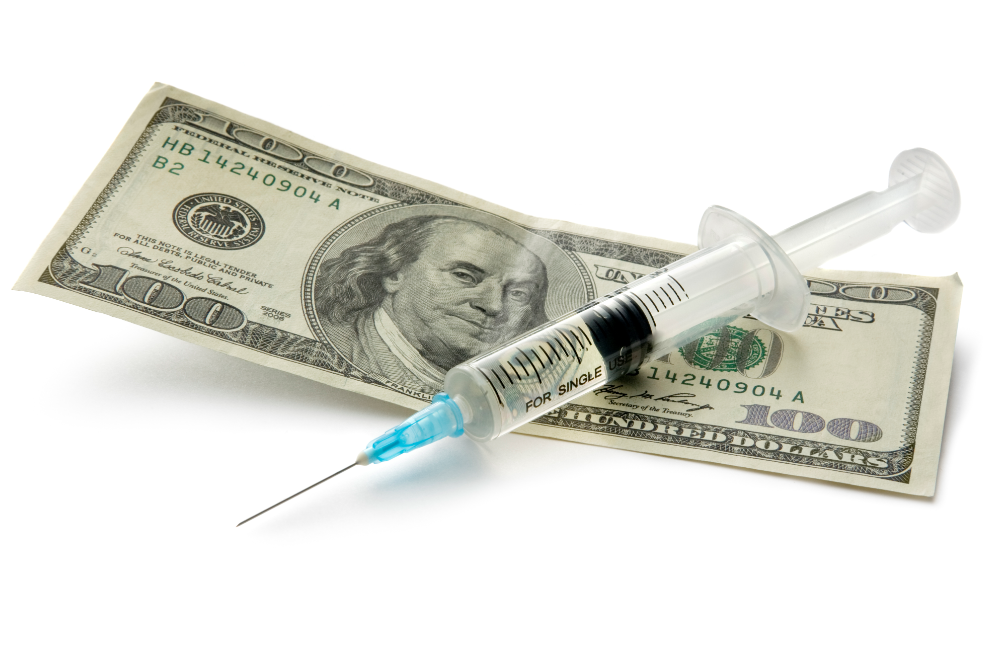
\includegraphics[width=0.9\linewidth]{Tex/logo.png}
\end{center}
\vspace{1cm}
%Supervisor's Details
\begin{center}
    {\LARGE Professor R. Burger\par}
    \vspace{1cm}
%Degree
    {\LARGE Behavioural Economics 871 Essay\par}
    \vspace{1cm}
%Institution
    {\LARGE 15 October 2021\par}
    \vspace{1cm}
%Date
    {\large }
%More
    {\normalsize }
%More
    {\normalsize }
\end{center}
\end{minipage}
\end{center}
\clearpage


\begin{frontmatter}  %

\title{}

% Set to FALSE if wanting to remove title (for submission)


\vspace{1cm}





\vspace{0.5cm}

\end{frontmatter}


\renewcommand{\contentsname}{Table of Contents}
{\tableofcontents}

%________________________
% Header and Footers
%%%%%%%%%%%%%%%%%%%%%%%%%%%%%%%%%
\pagestyle{fancy}
\chead{}
\rhead{}
\lfoot{}
\rfoot{\footnotesize Page \thepage}
\lhead{}
%\rfoot{\footnotesize Page \thepage } % "e.g. Page 2"
\cfoot{}

%\setlength\headheight{30pt}
%%%%%%%%%%%%%%%%%%%%%%%%%%%%%%%%%
%________________________

\headsep 35pt % So that header does not go over title




\newpage

\hypertarget{introduction-492}{%
\section{\texorpdfstring{Introduction \label{Introduction}
492}{Introduction  492}}\label{introduction-492}}

Coronavirus disease 2019 (COVID-19) has caused the largest public health
crisis, and economic disaster of the 21st century so far
(\protect\hyperlink{ref-bad}{Kadkhoda, 2021: 471}). According to the
\protect\hyperlink{ref-who}{World Health Organisation}
(\protect\hyperlink{ref-who}{2021}), COVID-19 has directly resulted in
4,859,277 deaths worldwide\footnote{As of 13 October 2021}, and its
impact on the global economy has been severe
(\protect\hyperlink{ref-bank}{World Bank, 2020}). Policymakers are in
urgent need of evidence-based strategies to contain the pandemic. As
\protect\hyperlink{ref-immun}{Fontanet \& Cauchemez}
(\protect\hyperlink{ref-immun}{2020: 583}) report, one critical
mechanism through which epidemics are controlled is through herd
immunity. Herd immunity arises when a sufficiently large proportion of
the population achieves individual immunity to an infectious disease
such that the transmission chain of the disease is halted
(\protect\hyperlink{ref-bad}{Kadkhoda, 2021: 471}). One method of
establishing herd immunity is through vaccination programs
(\protect\hyperlink{ref-immun}{Fontanet \& Cauchemez, 2020: 583}).
Preliminary empirical evidence shows that infection detection and
vaccination strategies could be critical tools in subduing COVID-19, for
example the study by \protect\hyperlink{ref-erad}{Aldila, Samiadji,
Simorangkir, Khosnaw \& Shahzad} (\protect\hyperlink{ref-erad}{2021})
finds COVID-19 vaccines to be effective in Jakarta, Indonesia. Leaders
of other countries have also implemented vaccine programs and the
\protect\hyperlink{ref-who}{World Health Organisation}
(\protect\hyperlink{ref-who}{2021}) reports that a total of
6,364,021,792 vaccine doses have been administered globally as of 10
October 2021.

In line with the international approach, South Africa has opted to issue
vaccines in addition to social distancing and lockdown measures. The
South African government has stated that it aims to have 67\% of the
population vaccinated by the end of 2021
(\protect\hyperlink{ref-herd}{Department of Health, 2021a}). However,
many South Africans are hesitant to get the COVID vaccine;
\protect\hyperlink{ref-stat}{Department of Health}
(\protect\hyperlink{ref-stat}{2021b}) records that only 25\% of South
Africa's adult population has been fully vaccinated as of 11 October
2021. \protect\hyperlink{ref-cram}{Burger, Maughan-Brown, Köhler,
English \& Tameris} (\protect\hyperlink{ref-cram}{2021}) compiled a
report, based on data from wave 5 of the NIDS-CRAM survey, and find that
that around 20\% of South Africans are concerned that COVID-19 vaccines
are not safe. The report also shows that relatively few people in the
sample registered to be vaccinated within two months after registration
opened. \protect\hyperlink{ref-cram}{Burger, Maughan-Brown, Köhler,
English \& Tameris} (\protect\hyperlink{ref-cram}{2021}) conclude that a
significant portion of South Africans still have to be convinced to take
the vaccine\footnote{A sentiment report from
  \protect\hyperlink{ref-report}{Department of Health}
  (\protect\hyperlink{ref-report}{2021c}) shows an interesting break
  down of different communities' beliefs surrounding the vaccine}. While
there are different ways to encourage vaccine uptake, such as mandatory
vaccination or lump-sum transfers, insights from behaviourial economics
could provide a more cost-effective solution: a vaccine lottery.

This essay\footnote{This essay was written using the package Texevier by
  \protect\hyperlink{ref-Texevier}{Katzke}
  (\protect\hyperlink{ref-Texevier}{2017})} proposes a field experiment
to investigate whether a vaccine lottery could improve vaccination rates
in South Africa. The experiment explores the effect of three different
lottery types - standard, regret and referral - on the take up of
vaccines. This essay is structured as follows. Section \ref{lit} briefly
reviews the relevant literature on behavioural economics and health
incentives. Section \ref{context} elaborates on the South African
context. Section \ref{design} describes the design of the experiment and
outlines the three types of treatment groups. Section \label{treat}
discusses how the treatment will be administered and how the data will
be collected. Lastly, section \ref{pre} gives a pre-analysis plan of the
empirical analysis that will be performed on the data, and the final
section (\ref{con}) concludes.

• a clear statement of the research question and motivation for why this
is interesting and important;

\hypertarget{behavioural-economics-and-health-incentives}{%
\section{\texorpdfstring{Behavioural Economics and Health Incentives
\label{lit}}{Behavioural Economics and Health Incentives }}\label{behavioural-economics-and-health-incentives}}

Health professionals and policymakers are increasingly turning to
behavioural economics to understand how people make health decisions and
how behavioural insights can be used to improve public health outcomes
(\protect\hyperlink{ref-health}{Loewenstein, Asch, Friedman, Melichar \&
Volpp, 2012: 1}). While neoclassical economics assumes that people are
perfectly rational agents, behavioural economics relaxes this assumption
and uses psychology and economic theory to create more realistic models
of human decision-making (\protect\hyperlink{ref-rabin}{Rabin, 2002}).
As Khaneman and Tversky show, people are subject to certain biases and
often make use of heuristics in their decision-making process, which can
lead to predictable errors in judgment
\protect\hyperlink{ref-prospect}{Kahneman \& Tversky}
(\protect\hyperlink{ref-prospect}{1979}). A large literature has
developed in the field of behavioural economics to investigate how these
biases can be combated and sub-optimal choices overcome to improve
welfare. \protect\hyperlink{ref-nudge}{Thaler \& Sunstein}
(\protect\hyperlink{ref-nudge}{2008}) introduced the idea of a
nudge\footnote{Nudge: an intervention that alters behaviour towards a
  desired action. In order for an intervention to qualify as a nudge, it
  should be cheap and easy to avoid \protect\hyperlink{ref-nudge}{Thaler
  \& Sunstein} (\protect\hyperlink{ref-nudge}{2008})} as a way to guide
people to make better choices. For example,
\protect\hyperlink{ref-nudge}{Thaler \& Sunstein}
(\protect\hyperlink{ref-nudge}{2008: 176}) proposed changing the default
option for organ donation in America to opt-in as opposed to explicit
consent. They found that many people who were willing to be organ donors
did not take the necessary steps, and that the registration process
appeared to deter otherwise willing donors. By changing the choice
architecture to presumed consent (with an easy opt-out option), there
would be more registered donors and more lives saved.

There are other empirical studies that
\protect\hyperlink{ref-flu}{Madrian} (\protect\hyperlink{ref-flu}{2014})

Nudges can be effective because people are influenced by stimuli that
are visible and new; thus, at least in theory, small changes can lead to
behavior modification. Several studies have found that simply prompting
(nudging) individuals to make a plan increases the probability of the
subject eventually engaging in the prompted health behavior, such as
immunizations, healthy eating, and cancer screening.25

For example, one study found that e-mailing patients appointment times
and locations for their next influenza vaccination increased vaccination
rates by 36\%.26 Another intervention was even simpler. Rather than
assigning a date and time for the patient to be vaccinated, patients
were simply mailed a card that asked the patient to write down the day
or day and time they planned to get the influenza vaccine (they were
also sent the day and time of the free influenza vaccine clinics).27
Relative to a control condition (people who only received the
information about the day and time of the clinics), those prompted to
write down the day and time they planned to get the influenza vaccine
were 4.2 percentage points (12.7\%) more likely to receive the vaccine
at those clinics. Those prompted to write down the date but not the time
were not significantly more likely to be vaccinated at the clinics.

A lottery system can be a cost-effective mechanism for changing
behaviour compared to direct transfers because people tend to overweight
small probabilities. Due to this nonlinear probability weighting, an
individual overestimates her chances of winning a lottery.

chance for regret, which behavioral scientists have found to be
particularly motivating. Specifically, our ``regret lottery''
capitalizes on people's general desire to avoid losses to a greater
degree than seeking equivalent gains (12) and to avoid anticipated
regret (20-25).

It is not unprecedented to use lotteries in public health interventions.
To the best of my knowledge, this experiment would be the first
randomized field experiment to assess the impact of lotteries on
COVID-19 vaccine take-up in South Africa. Several papers show that
regret lotteries can improve health outcomes, such as
\protect\hyperlink{ref-regr}{Husain, Diaz, Schwartz, Parsons, Burg,
Davidson \& Kronish} (\protect\hyperlink{ref-regr}{2019}) and
\protect\hyperlink{ref-adhere}{Humphrey, Small, Jensen, Volpp, Asch, Zhu
\& Troxel} (\protect\hyperlink{ref-adhere}{2019})

Loss aversion, regret avoidance, social preferences referral incentives

Individuals have a tendency to overweight small probabilities and this
overestimate their chances of winning a lottery. behavioural economics
theory and

research gap your experiment will address;

This paper addresses the gap pf vaccine lotteries in SA.

\hypertarget{the-south-african-context}{%
\section{\texorpdfstring{The South African Context
\label{context}}{The South African Context }}\label{the-south-african-context}}

There are currently four vaccines which have been approved by the South
African Health Products Regulatory Authority for use in South Africa:
Johnson \& Johnson (J\&J), Pfizer, Sinovac and AstraZeneca. The two main
vaccines being rolled out in South Africa are the J\&J and Pfizer, which
are both available for free. Vaccines are currently only available to
individuals over the age of 18. The J\&J vaccine only requires 1 dose;
and the Pfizer vaccine requires two doses, 6 weeks apart. For the
purposes of this field experiment, \emph{fully vaccinated} refers to an
individual who has had either 1 J\&J shot, or both shots of the Pfizer
vaccine. \emph{Vaccinated} refers to an individual who has had 1 shot of
either vaccine.

According to \protect\hyperlink{ref-stat}{Department of Health}
(\protect\hyperlink{ref-stat}{2021b}), 34\% of South Africans are
vaccinated, while only 25\% are fully vaccinated.

\begin{table}[H]
\centering
\begin{tabular}{llll}
  \toprule
Province & Total Adults Vaccinated & Adult Population & Percentage Vaccinated \\ 
  \midrule
Eastern Cape & 1 603 045 & 4 099 543 & 39\% \\ 
  Free State & 735 696 & 1 914 521 & 38\% \\ 
  Gauteng & 3 523 373 & 11 311 326 & 31\% \\ 
  KwaZulu-Natal & 2 170 526 & 7 219 795 & 30\% \\ 
  Limpopo & 1 437 846 & 3 695 801 & 39\% \\ 
  Mpumalanga & 831 759 & 3 039 520 & 27\% \\ 
  North West & 835 206 & 2 693 247 & 31\% \\ 
  Northern Cape & 290 962 & 847 545 & 34\% \\ 
  Western Cape & 2 141 933 & 4 976 903 & 43\% \\ 
  Total & 13 570 346 & 39 798 201 & 34\% \\ 
   \bottomrule
\end{tabular}
\caption{Vaccination Statistics \label{tab1}} 
\end{table}

gambling in SA

\hypertarget{experiment-design}{%
\section{\texorpdfstring{Experiment Design
\label{design}}{Experiment Design }}\label{experiment-design}}

• a clear description of the experimental design and the theory of
change;

The field experiment is designed to address the research question: could
a vaccine lottery improve vaccination rates in South Africa?

The sample used will be the same sample used for the Coronavirus Rapid
Mobile Survey (NIDS-CRAM). NIDS-CRAM was created in response to the
pandemic as a way to build a representative data set of the South
African population to inform decision-making
(\protect\hyperlink{ref-nids}{Ingle, 2021}). Thus far, there have been
five waves of NIDS-CRAM surveys, with wave 5 comprising a sample of
5,862 people being surveyed during 6 April to 11 May 2021
(\protect\hyperlink{ref-nids}{Ingle}
(\protect\hyperlink{ref-nids}{2021}) p.14). Wave 3 consisted of a total
of 8,157 potential participants, of which 6,130 were successfully
interviewed. For the purposes of this field experiment, the 8,157 people
from Wave 3 will be contacted and asked to participate in the
experiment. It seems reasonable to expect between 5,500 and 6,200 people
to participate, given the previous rates of attrition experienced in
NIDS-CRAM.

The NIDS-CRAM sample will then be split into 4 groups of equal size.
Assuming a conservative sample size of 5,500, each of the 4 groups will
comprise 1,375 individuals. \protect\hyperlink{ref-random}{Duflo,
Glennerster \& Kremer} (\protect\hyperlink{ref-random}{2007}) which will
be randomised using the randomisation technique as proposed by @. The
first group is the control group, where individuals will not be entered
into any vaccine lottery. The other 3 groups are will receive different
lottery treatments, which are explained below. There will be 3 monthly
lotteries for each treatment group, which will run simultaneously. Thus,
in total there will be 9 lotteries for this field experiment, with 3
lotteries every month. Each lottery will award a cash prize of
R1,000,000.

NIDS-CRAM is a special follow-up survey of a subsample of adults from
households that were part of the last wave (2017) of the National Income
Dynamics Study (NIDS). NIDS was a large-scale longitudinal survey, run
by the Southern Africa Labour and Development Research Unit (SALDRU),
that tracked the social and economic well-being of South Africans from
2008 up to 2017. SALDRU (based at the University of Cape Town) was
responsible for the NIDS-CRAM survey data collection, quality assurance
and production. The NIDS-CRAM survey instrument includes a wide range of
questions on income and employment, sociodemographic characteristics,
and household welfare. This paper draws on questions about vaccine
acceptance that were included in Waves 4 and 5 of the NIDS-CRAM survey.
Wave 4 was conducted from 2 February to 10 March 2021 with a sample of
4,792 individuals, and Wave 5 was conducted from 6 April to 11 May 2021
with a sample of 4,996. Compared to NIDS-CRAM Wave 1 (May and June
2020), Wave 4 had 31\% attrition and Wave 5 had 28\% attrition.

For the first treatment group, if an individual has received a
vaccination shot\footnote{An individual only need a receive one shot of
  any vaccine - receiving the first shot of the Pfizer qualifies an
  individual for that month's lottery} within a given month, she will be
entered into that month's vaccine lottery. At the end of the month, a
winner is randomly selected from the lottery pool. Once it is verifed
that the winner has been vaccinated, she will be privately contacted and
will receive a cash prize. It will then be announced via sms to everyone
in the treatment group (group 1) that the lottery has been won, the
amount of the lottery prize, and the winner's province.

Following the approach of \protect\hyperlink{ref-regret}{Gandhi,
Milkman, Ellis, Graci, Gromet, Mobarak, Buttenheim, Duckworth, Pope,
Stanford, Thaler \& Volpp} (\protect\hyperlink{ref-regret}{2021}), the
second lottery is a ``regret lottery''. Every individual in the sample
is entered into a monthly lottery but an individual may only claim her
prize if she has been vaccinated (i.e.~had at least 1 shot of any
vaccine). At month end, a winner is randomly drawn from the lottery
pool. If the winner has been vaccinated, she will be privately notified
and will receive a cash prize. It will then be announced via sms to
everyone in the treatment group (group 3) that the lottery has been won,
the amount of the cash prize, the winner's province and a reminder that
only vaccinated individuals are eligible to win the lottery.

The final treatment is a ``referral lottery''. An individual is entered
into the monthly lottery if 2 conditions are met: he is vaccinated, and
he refers a friend to get vaccinated and the friend gets vaccinated.
Both the individual from the sample and his friend are entered into the
lottery. At the end of the month, a winner is selected, verified to be
vaccinated and privately informed. An SMS is sent out to the treatment
group with the same information as for group 2 and group 3, in addition
to a message thanking the sample for protecting their friends as well as
a reminder that they can refer more friends to be eligible for the
following month's lottery.

Including an SMS after the lottery has won serves as a reminder that
there is a

Table \ref{tab2} summarises the different treatments administered.

\begin{table}[H]
\centering
\begin{tabular}{ll}
  \toprule
Group & Treatment \\ 
  \midrule
Control & No lottery \\ 
  Group 1 & Individual is entered into a lottery once they are vaccinated \\ 
  Group 2 & Everyone in the group is entered into a lottery; only vaccinated individuals can claim the prize \\ 
  Group 3 & Individual is entered if she is vaccinated and refers a friend, who gets vaccinated \\ 
   \bottomrule
\end{tabular}
\caption{Treatment Summary \label{tab2}} 
\end{table}

Many South Africans are hesitant to get the COVID vaccine. As STATSA
shows, amount of people have received the vaccine so far. Critical to
reach herd immunity is improving vaccination rates. In order to improve
the take-up of vaccinations, a field experiment designed around a
vaccination lottery is proposed. While some governments have considered
and experimented with lump-sum payments, behavioural economics could
provide a more cost-effective solution. Individuals have a tendency to
overweight small probabilities and this overestimate their chances of
winning a lottery. In South Africa,

Theory: overweight small probabilities, gambling, social preferences,
regret avoidance Empirical: vaccine field designs, lottery incentives,
regret lottery incentives Several authors have experimented with
lotteries as an incentive for vaccinations, although there have been no
studies as of yet on the South African population. Probles with vaccine
studies: too few participants. A larger study could fill this gap in the
literature.

\hypertarget{treatment-and-data}{%
\section{\texorpdfstring{Treatment and Data
\label{treat}}{Treatment and Data }}\label{treatment-and-data}}

• an explanation of how the treatments will be administered and data
gathered (including proposed partner institutions);

The CRAM survey exists to provide monthly nationally-representative data
on key outcomes such as unemployment, household income, child hunger and
access to government grants.

Partner with NIDS, department of health, vaccine administer, funding
data collected at vaccine add 3 questions to NIDS data cram

\hypertarget{pre-analysis-plan}{%
\section{\texorpdfstring{Pre-analysis plan
\label{pre}}{Pre-analysis plan }}\label{pre-analysis-plan}}

• a pre-analysis plan of the empirical analysis that will be performed
on the data.

Overview In this field experiment, a person who refers his/her friend to
receive a vaccine would be entered into a lucky draw, with a monetary
prize, created by the government. The purpose behind this nudge is to
encourage people who would otherwise not have got a Covid vaccine, to do
so. The hypothesis is that there should be an increase in the total
number of people receiving a Covid vaccine after the nudge is
implemented. Increasing the number of vaccinations is important as
medical research shows that vaccines decrease the probability of
contracting Covid-19 and are also effective at reducing the severity of
the symptoms of the virus for those who do contract it. The Nudge The
nudge addresses behaviour by creating an environment where there is
social pressure to get a vaccine (if I wanted to enter the lucky draw, I
would pressure my friend into getting the vaccine). It is also likely
that if a person asks her friend to get the vaccine so she can enter the
lucky draw, she will reciprocate and get the vaccine as well so that her
friend may enter the draw, which will also increase the number of people
getting vaccinated. For the vaccines that require two doses
(e.g.~Pfizer), a person's name could be withdrawn, if the second shot is
not given within a certain amount of time. This makes use of loss
aversion, where people who already have their names in the draw feel the
pain of having their names withdrawn more intensely than the pleasure of
having their names added a second time to the draw for getting their
second shot. Target Group The lucky draw is anticipated to attract
people who are risk-on (they enjoy gambling, and are less worried about
getting vaccinated), and poorer individuals for whom winning money is
more attractive. These target groups are desirable as they are less
likely to get the vaccine, and the government would like to maximise the
number of vaccinated people. Additionally, if there are individuals who
want to be vaccinated but procrastinate getting the vaccine (e.g.~naïve
hyperbolic discounters), setting a deadline for the lucky draw could
increase the utility of getting the vaccine earlier enough to overcome
the procrastination problem. There is no downside or extra cost for
having people enter the lucky draw who would otherwise still have got
the vaccine. Proposed Partner Institutions This field experiment would
be in collaboration with the South African government and facilities
that conduct vaccinations (e.g.~Clicks). The government would be where
the data is centralized and the administers of vaccines would all be
data collection nodes. After a person has received a vaccine, the
administer would ask if the person received a referral for the shot, and
then note the ID number of the friend in addition to the individual's
details.

Data Collection There is a data collection system already set up at the
vaccination sites so this extra data point would not be difficult to
collect within the current tracking system. Depending on costs, the
referral friend could be sent an sms thanking her for caring about
others and getting them vaccinated, and letting her know that she has
been entered into the draw. This is a positive reinforcement technique
and shows people that the government is following up on their promise.
This acknowledgement and transparency is expected to encourage more
referrals. Once the lucky draw has been concluded, the data can be
analysed, the purpose of which is to uncover whether the nudge increased
vaccinations.

\begin{quote}
I suggest renaming the top line after @article, as done in the template
ref.bib file, to something more intuiti
\end{quote}

\begin{figure}[H]

{\centering \includegraphics{Write_Up_files/figure-latex/Figure1-1} 

}

\caption{Caption Here \label{Figure1}}\label{fig:Figure1}
\end{figure}

To reference calculations \textbf{in text}, \emph{do this:} From table
\ref{tab1} we see the average value of mpg is 20.98.

\begingroup\fontsize{12pt}{13pt}\selectfont
\begin{longtable}{rrrrrrrrrrr}
\caption{Long Table Example} \\ 
  \toprule
mpg & cyl & disp & hp & drat & wt & qsec & vs & am & gear & carb \\ 
  \hline 
\endhead 
\hline 
{\footnotesize Continued on next page} 
\endfoot 
\endlastfoot 
 \midrule
21.00 & 6.00 & 160.00 & 110.00 & 3.90 & 2.62 & 16.46 & 0.00 & 1.00 & 4.00 & 4.00 \\ 
  21.00 & 6.00 & 160.00 & 110.00 & 3.90 & 2.88 & 17.02 & 0.00 & 1.00 & 4.00 & 4.00 \\ 
  22.80 & 4.00 & 108.00 & 93.00 & 3.85 & 2.32 & 18.61 & 1.00 & 1.00 & 4.00 & 1.00 \\ 
  21.40 & 6.00 & 258.00 & 110.00 & 3.08 & 3.21 & 19.44 & 1.00 & 0.00 & 3.00 & 1.00 \\ 
  18.70 & 8.00 & 360.00 & 175.00 & 3.15 & 3.44 & 17.02 & 0.00 & 0.00 & 3.00 & 2.00 \\ 
  18.10 & 6.00 & 225.00 & 105.00 & 2.76 & 3.46 & 20.22 & 1.00 & 0.00 & 3.00 & 1.00 \\ 
  14.30 & 8.00 & 360.00 & 245.00 & 3.21 & 3.57 & 15.84 & 0.00 & 0.00 & 3.00 & 4.00 \\ 
  24.40 & 4.00 & 146.70 & 62.00 & 3.69 & 3.19 & 20.00 & 1.00 & 0.00 & 4.00 & 2.00 \\ 
  22.80 & 4.00 & 140.80 & 95.00 & 3.92 & 3.15 & 22.90 & 1.00 & 0.00 & 4.00 & 2.00 \\ 
  19.20 & 6.00 & 167.60 & 123.00 & 3.92 & 3.44 & 18.30 & 1.00 & 0.00 & 4.00 & 4.00 \\ 
  17.80 & 6.00 & 167.60 & 123.00 & 3.92 & 3.44 & 18.90 & 1.00 & 0.00 & 4.00 & 4.00 \\ 
  16.40 & 8.00 & 275.80 & 180.00 & 3.07 & 4.07 & 17.40 & 0.00 & 0.00 & 3.00 & 3.00 \\ 
  17.30 & 8.00 & 275.80 & 180.00 & 3.07 & 3.73 & 17.60 & 0.00 & 0.00 & 3.00 & 3.00 \\ 
  15.20 & 8.00 & 275.80 & 180.00 & 3.07 & 3.78 & 18.00 & 0.00 & 0.00 & 3.00 & 3.00 \\ 
  10.40 & 8.00 & 472.00 & 205.00 & 2.93 & 5.25 & 17.98 & 0.00 & 0.00 & 3.00 & 4.00 \\ 
  10.40 & 8.00 & 460.00 & 215.00 & 3.00 & 5.42 & 17.82 & 0.00 & 0.00 & 3.00 & 4.00 \\ 
  14.70 & 8.00 & 440.00 & 230.00 & 3.23 & 5.34 & 17.42 & 0.00 & 0.00 & 3.00 & 4.00 \\ 
  32.40 & 4.00 & 78.70 & 66.00 & 4.08 & 2.20 & 19.47 & 1.00 & 1.00 & 4.00 & 1.00 \\ 
  30.40 & 4.00 & 75.70 & 52.00 & 4.93 & 1.61 & 18.52 & 1.00 & 1.00 & 4.00 & 2.00 \\ 
  33.90 & 4.00 & 71.10 & 65.00 & 4.22 & 1.83 & 19.90 & 1.00 & 1.00 & 4.00 & 1.00 \\ 
  21.50 & 4.00 & 120.10 & 97.00 & 3.70 & 2.46 & 20.01 & 1.00 & 0.00 & 3.00 & 1.00 \\ 
  15.50 & 8.00 & 318.00 & 150.00 & 2.76 & 3.52 & 16.87 & 0.00 & 0.00 & 3.00 & 2.00 \\ 
  15.20 & 8.00 & 304.00 & 150.00 & 3.15 & 3.44 & 17.30 & 0.00 & 0.00 & 3.00 & 2.00 \\ 
  13.30 & 8.00 & 350.00 & 245.00 & 3.73 & 3.84 & 15.41 & 0.00 & 0.00 & 3.00 & 4.00 \\ 
  19.20 & 8.00 & 400.00 & 175.00 & 3.08 & 3.85 & 17.05 & 0.00 & 0.00 & 3.00 & 2.00 \\ 
  27.30 & 4.00 & 79.00 & 66.00 & 4.08 & 1.94 & 18.90 & 1.00 & 1.00 & 4.00 & 1.00 \\ 
  26.00 & 4.00 & 120.30 & 91.00 & 4.43 & 2.14 & 16.70 & 0.00 & 1.00 & 5.00 & 2.00 \\ 
  30.40 & 4.00 & 95.10 & 113.00 & 3.77 & 1.51 & 16.90 & 1.00 & 1.00 & 5.00 & 2.00 \\ 
  15.80 & 8.00 & 351.00 & 264.00 & 4.22 & 3.17 & 14.50 & 0.00 & 1.00 & 5.00 & 4.00 \\ 
  19.70 & 6.00 & 145.00 & 175.00 & 3.62 & 2.77 & 15.50 & 0.00 & 1.00 & 5.00 & 6.00 \\ 
  15.00 & 8.00 & 301.00 & 335.00 & 3.54 & 3.57 & 14.60 & 0.00 & 1.00 & 5.00 & 8.00 \\ 
  21.40 & 4.00 & 121.00 & 109.00 & 4.11 & 2.78 & 18.60 & 1.00 & 1.00 & 4.00 & 2.00 \\ 
   \bottomrule
\end{longtable}
\endgroup

\hfill

\hypertarget{conclusion}{%
\section{\texorpdfstring{Conclusion
\label{con}}{Conclusion }}\label{conclusion}}

\newpage

\hypertarget{references}{%
\section*{References}\label{references}}
\addcontentsline{toc}{section}{References}

\hypertarget{refs}{}
\begin{CSLReferences}{1}{0}
\leavevmode\hypertarget{ref-erad}{}%
Aldila, D., Samiadji, B.M., Simorangkir, G.M., Khosnaw, S.H. \& Shahzad,
M. 2021. Impact of early detection and vaccination strategy in COVID-19
eradication program in jakarta, indonesia. \emph{BMC Research Notes}.
14(1):1--7.

\leavevmode\hypertarget{ref-cram}{}%
Burger, R., Maughan-Brown, B., Köhler, T., English, R. \& Tameris, M.
2021. \emph{A shot in the arm for south africa - increased openness to
accepting a COVID-19 vaccine: Evidence from NIDS-CRAM waves 4 and 5}.
National Income Dynamics Study (NIDS) -- Coronavirus Rapid Mobile Survey
(CRAM). {[}Online{]}, Available: \url{https://cramsurvey.org/reports/}.

\leavevmode\hypertarget{ref-stat}{}%
Department of Health. 2021b. \emph{Latest vaccine statistics}. Republic
of South Africa. {[}Online{]}, Available:
\url{https://sacoronavirus.co.za/latest-vaccine-statistics/}.

\leavevmode\hypertarget{ref-herd}{}%
Department of Health. 2021a. \emph{COVID-19 coronavirus vaccine}.
Republic of South Africa. {[}Online{]}, Available:
\url{https://www.gov.za/covid-19/vaccine/vaccine}.

\leavevmode\hypertarget{ref-report}{}%
Department of Health. 2021c. \emph{South africa COVID-19 and vaccine
social listening report}. Republic of South Africa. {[}Online{]},
Available:
\url{https://sacoronavirus.b-cdn.net/wp-content/uploads/2021/10/SA-social-listening-report-5-Oct-2021.pdf}.

\leavevmode\hypertarget{ref-random}{}%
Duflo, E., Glennerster, R. \& Kremer, M. 2007. Using randomization in
development economics research: A toolkit. \emph{Handbook of development
economics}. 4:3895--3962.

\leavevmode\hypertarget{ref-immun}{}%
Fontanet, A. \& Cauchemez, S. 2020. COVID-19 herd immunity: Where are
we? \emph{Nature reviews. Immunology}. 20:583--584.

\leavevmode\hypertarget{ref-regret}{}%
Gandhi, L., Milkman, K.L., Ellis, S., Graci, H., Gromet, D., Mobarak,
R., Buttenheim, A., Duckworth, A., et al. 2021. An experiment evaluating
the impact of large-scale, high-payoff vaccine regret lotteries.
{[}Online{]}, Available: \url{http://dx.doi.org/10.2139/ssrn.3904365}.

\leavevmode\hypertarget{ref-adhere}{}%
Humphrey, C.H., Small, D.S., Jensen, S.T., Volpp, K.G., Asch, D.A., Zhu,
J. \& Troxel, A.B. 2019. Modeling lottery incentives for daily
adherence. \emph{Statistics in Medicine}. 38(15):2847--2867.

\leavevmode\hypertarget{ref-regr}{}%
Husain, S.A., Diaz, K.M., Schwartz, J.E., Parsons, F.E., Burg, M.M.,
Davidson, K.W. \& Kronish, I.M. 2019. Behavioral economics
implementation: Regret lottery improves health patient study adherence.
\emph{Contemporary Clinical Trials Communications}. 15:100387.

\leavevmode\hypertarget{ref-nids}{}%
Ingle, B., K. 2021. \emph{National income dynamics study -- coronavirus
rapid mobile survey (NIDS-CRAM) 2020 - 2021 panel user manual.} Cape
Town: Southern Africa Labour; Development Research Unit: Bureau for
Economic Research.

\leavevmode\hypertarget{ref-bad}{}%
Kadkhoda, K. 2021. Herd immunity to COVID-19: Alluring and elusive.
\emph{American Journal of Clinical Pathology}. 155(4):471--472.

\leavevmode\hypertarget{ref-fast}{}%
Kahneman, D. 2011. \emph{Thinking, fast and slow}. Macmillan.

\leavevmode\hypertarget{ref-prospect}{}%
Kahneman, D. \& Tversky, A. 1979. Prospect theory: An analysis of
decision under risk. \emph{Econometrica}. 47(2):363--391.

\leavevmode\hypertarget{ref-Texevier}{}%
Katzke, N.F. 2017. \emph{{Texevier}: {P}ackage to create elsevier
templates for rmarkdown}. Stellenbosch, South Africa: Bureau for
Economic Research.

\leavevmode\hypertarget{ref-health}{}%
Loewenstein, G., Asch, D., Friedman, J., Melichar, L. \& Volpp, K. 2012.
Can behavioural economics make us healthier? \emph{BMJ (Clinical
research ed.)}. 344:e3482.

\leavevmode\hypertarget{ref-flu}{}%
Madrian, B. 2014. Applying insights from behavioral economics to policy
design. {[}Online{]}, Available: \url{http://dx.doi.org/10.3386/w20318}.

\leavevmode\hypertarget{ref-rabin}{}%
Rabin, M. 2002. A perspective on psychology and economics.
\emph{European economic review}. 46(4-5):657--685.

\leavevmode\hypertarget{ref-nudge}{}%
Thaler, R. \& Sunstein, C. 2008. \emph{Nudge: Improving decisions about
health, wealth, and happiness.} New Haven, CT: Yale University Press.

\leavevmode\hypertarget{ref-khan}{}%
Tversky, A. \& Kahneman, D. 1974. Judgment under uncertainty: Heuristics
and biases. \emph{Science}. 185(4157):1124--1131.

\leavevmode\hypertarget{ref-bank}{}%
World Bank. 2020. \emph{The global economic outlook during the COVID-19
pandemic: A changed world}. {[}Online{]}, Available:
\url{https://www.worldbank.org/en/news/feature/2020/06/08/the-global-economic-outlook-during-the-covid-19-pandemic-a-changed-world}.

\leavevmode\hypertarget{ref-who}{}%
World Health Organisation. 2021. \emph{WHO coronavirus (COVID-19)
dashboard}. {[}Online{]}, Available:
\url{https://covid19.who.int/table}.

\end{CSLReferences}

\hypertarget{appendix}{%
\section*{Appendix}\label{appendix}}
\addcontentsline{toc}{section}{Appendix}

\hypertarget{appendix-a}{%
\subsection*{Appendix A}\label{appendix-a}}
\addcontentsline{toc}{subsection}{Appendix A}

Some appendix information here

\hypertarget{appendix-b}{%
\subsection*{Appendix B}\label{appendix-b}}
\addcontentsline{toc}{subsection}{Appendix B}

\bibliography{Tex/ref}





\end{document}
